\documentclass[a4paper,openright,12pt,spanish]{book}

% Cargar preámbulo
% Carga de paquetes
\usepackage[spanish,es-noshorthands,es-nosectiondot]{babel}
\selectlanguage{spanish}
\usepackage[utf8]{inputenc} % Codificación UTF-8
\usepackage[T1]{fontenc}    % Salida de caracteres
\usepackage{amsmath, amssymb, amsthm, mathtools} % Matemáticas
\usepackage{amsfonts,latexsym,cancel}
\usepackage{graphicx}       % Imágenes
\usepackage{tikz}  % Crear imágenes
\usepackage[figurename=Fig.]{caption}

\usepackage[breaklinks=true]{hyperref}       % Hipervínculos
\usepackage{xcolor}         % Colores
\usepackage{geometry}       % Márgenes
%\usepackage[total={6.3in,9in},top=1in,left=1.4in]{geometry}  %Márgenes
\usepackage{fancyhdr}       % Encabezados y pies de página

\usepackage{enumerate}
\usepackage{array}

%\usepackage{appendix}

%%%%%%%%%%%% Indices alfabetico, glosario, simbolos %%%%%%%%%%%
\usepackage{makeidx} % Permite crear índices
\makeindex 
\usepackage[totoc]{idxlayout}
%%%%%%%%%%%%%%%%%%%%%%%%%%%%% GLosarios %%%%%%%%%%%%%%%%%%%%%%%%%%%
\usepackage[nonumberlist,acronym,toc]{glossaries}
\makeglossaries

%%%%%%%%%%%%%%%%% Para agregar a la tabla de contenidos:
%\usepackage[nottoc,notbib]{tocbibind}


%%%%%%%%%%%%%%%%%%%%%%%%% Tabla de contenidos%%%%%%%%%%%%%%%%%%%
\usepackage{tocloft}

%Cambiar título del índice de contenidos:
\renewcommand{\contentsname}{Índice}
% Cambiar profundidad del índice:
\setcounter{tocdepth}{2} % Incluye hasta 0: capítulos; 1: secciones; 2: subsecciones; 3: subsubsecciones; así sucesivamente

% Cambiar el tamaño de los títulos en el índice de contenidos
\renewcommand{\cfttoctitlefont}{\huge\bfseries}
\renewcommand{\cftchapfont}{\bfseries}
\renewcommand{\cftsecfont}{\itshape}
\renewcommand{\cftchappagefont}{\bfseries}
\renewcommand{\cftsecpagefont}{\itshape}


%%%%%%%%%% Índice de resultados importantes %%%%%%%%%%%%%%%%%%%%
\renewcommand{\indexname}{Índice Resultados importantes} %Renombrar el índice alfabético




\usepackage{emptypage}
\usepackage{float}
\usepackage{setspace}
\usepackage{cases}


% Configuración de márgenes
\geometry{margin=1in}
\setlength{\headheight}{15.35403pt}
% Estilo de encabezado
\pagestyle{fancy}
\fancyhf{}
\fancyhead[L]{\leftmark}
\fancyhead[R]{\thepage}

% Cargar estilos personalizados
% Cambiar fuentes para teoremas y demostraciones
\usepackage{lmodern}
\usepackage{titlesec}

% Estilo para teoremas
\newtheoremstyle{mytheorem}
  {10pt} % Espacio arriba
  {10pt} % Espacio abajo
  {\itshape} % Fuente del cuerpo
  {} % Sangría
  {\bfseries\color{blue}} % Fuente del título
  {} % Puntuación tras el título
  { } % Espacio tras el título
  {%
    \thmname{#1}~\thmnumber{#2}%
    \if\relax\detokenize{#3}\relax % Comprueba si la nota está vacía
    .\else~(\thmnote{#3}).\fi
  } % Formato del título

% Estilos numerados
\theoremstyle{mytheorem}
\newtheorem{theo}{Teorema}[chapter]
\newtheorem{lemma}[theo]{Lema}
\newtheorem{corol}[theo]{Corolario}
\newtheorem{conje}[theo]{Conjetura}
\newtheorem{ejem}{Ejemplo}[chapter]
\newtheorem{ejer}{Ejercicio}[chapter]

% Estilo para definiciones
\newtheoremstyle{mydefinition}
  {10pt}
  {10pt}
  {\normalfont} % Fuente normal (sin cursiva)
  {}
  {\bfseries\color{teal}}
  {}
  { }
  {%
    \thmname{#1}~\thmnumber{#2}%
    \if\relax\detokenize{#3}\relax % Comprueba si la nota está vacía
    \else~(\thmnote{#3}).\fi
  } % Formato del título

\theoremstyle{mydefinition}
\newtheorem*{defi}{Definición.}

% Estilo para demostraciones
\newtheoremstyle{mydemostration}
  {10pt}
  {10pt}
  {\normalfont} % Fuente normal (sin cursiva)
  {}
  {\bfseries}
  {}
  { }
  {\thmname{#1}~\thmnumber{#2}~\thmnote{(#3)}}

\theoremstyle{mydemostration}
\newtheorem*{dem}{Demostración.}
\renewcommand{\qedsymbol}{$\blacksquare$}
\AtEndEnvironment{dem}{\null\hfill\qedsymbol}
\newtheorem*{pd}{\textbf{P.D.}}

% Estilos no numerados
\theoremstyle{remark}
\newtheorem*{obs}{\textbf{Observación}}
\newtheorem*{notacion}{\textbf{Notación}}
\newtheorem*{afir}{\textbf{Afirmación}}



% Definir comandos personalizados
\newcommand{\R}{\mathbb{R}} % Conjunto de los números reales
\newcommand{\Z}{\mathbb{Z}} % Conjunto de los números enteros
\newcommand{\N}{\mathbb{N}} % Conjunto de los números naturales
\newcommand{\Q}{\mathbb{Q}} % Conjunto de los números racionales
\newcommand{\C}{\mathbb{C}} % Conjunto de los números complejos
\newcommand{\T}{\mathbb{T}} % El toro en C 
\newcommand{\Om}{\Omega} % Omega
\newcommand{\abs}[1]{\left\lvert#1\right\rvert} % Valor absoluto
\newcommand{\norm}[1]{\left\lVert#1\right\rVert} % Norma
\newcommand{\set}[1]{\left\{#1\right\}} % Conjunto
\newcommand{\inner}[2]{\langle#1, #2\rangle} % Producto interno

\newcommand{\derDefi}{\vcentcolon =} % Definición derecha :=
\newcommand{\izqDefi}{= \vcentcolon } % Definición inversa =:
\newcommand{\tq}{\, : \,} % tal que en conjuntos
\newcommand{\Real}{\mathtt{Re}} % Parte real de un complejo
\newcommand{\Imag}{\mathtt{Im}} % Parte imaginaria de un complejo
\newcommand*\conj[1]{\overline{#1}}  % Conjugado de un complejo


\newcommand*\closureSet[1]{\overline{#1}}  % Cerradura de un conjunto
%%% Acento para interior de conjuntos:
\DeclareFontFamily{U}{mathb}{\hyphenchar\font45}
\DeclareFontShape{U}{mathb}{m}{n}{ <-6> matha5 <6-7> matha6 <7-8>
mathb7 <8-9> mathb8 <9-10> mathb9 <10-12> mathb10 <12-> mathb12 }{}
\DeclareSymbolFont{mathb}{U}{mathb}{m}{n}

\DeclareMathAccent{\interiorSet}{0}{mathb}{"38}

\DeclareFontFamily{U}{mathb}{\hyphenchar\font45}
\DeclareFontShape{U}{mathb}{m}{n}{ <-6> matha5 <6-7> matha6 <7-8>
mathb7 <8-9> mathb8 <9-10> mathb9 <10-12> mathb10 <12-> mathb12 }{}
\DeclareSymbolFont{mathb}{U}{mathb}{m}{n}

%% Fin de acento para interior

\newcommand{\titlepageAMS}{
  \begin{titlepage}
    \centering
    \vspace*{2cm}
    {\Huge\bfseries \textsf{Notas de Variable Compleja}}\\[1cm]
    %{\Large\bfseries \textsf{César A. Díaz M.}}\\[3cm]
    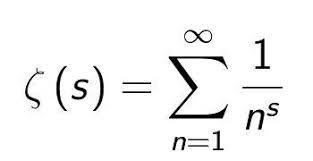
\includegraphics[width=0.3\textwidth]{images/logo_1.jpg}\\[2cm]
    {\large \textit{Publicación independiente}}\\[0.5cm]
    {\large \textit{\today}}\\[5cm]
    %\textsf{Con el apoyo de la comunidad matemática}\\[1cm]
    \vfill
  \end{titlepage}
}

% tikz_complejo.tex
%\usepackage{tikz}
%\usepackage{amsmath}
\usetikzlibrary{calc}
\usetikzlibrary{positioning}

% Estilo base para el plano complejo
\tikzset{
  complejo/.style={
    thick,
    opacity = 0.7,
    ->,
    >=stealth
  },
  punto/.style={
    circle,
    fill,
    inner sep=1pt
  },
  discoabierto/.style={
    draw=blue, thick, dashed, fill=blue!20, opacity=0.3
  },
  discocerrado/.style={
    draw=blue, thick, solid, fill=blue!20, opacity=0.4
  },
  regionConexa/.style={
    green!50, opacity=0.5, thick
  }
}

% Comando para dibujar el plano complejo
\newcommand{\planoComplejo}[1][]{
  \draw[complejo] (-3,0) -- (3,0) node[right] {\(x\)};
  \draw[complejo] (0,-3) -- (0,3) node[above] {\(y\)};
  % Opcional: título
  \ifx&#1&\else
    \node at (2.5,2.7) {#1};
  \fi
}

% Comando para dibujar el semi plano superior complejo
\newcommand{\semiPlanoComplejo}[1][]{
  \draw[complejo] (-3,0) -- (3,0) node[right] {\(x\)};
  \draw[complejo] (0,-0.5) -- (0,3) node[above] {\(y\)};
  % Opcional: título
  \ifx&#1&\else
    \node at (2.5,2.7) {#1};
  \fi
}

% Comando para dibujar el semi plano superior complejo con origen en punto dado
\newcommand{\semiPlanoComplejoCentrado}[2]{
  \draw[complejo] (#1 - 2.5,#2) -- (#1 + 2.5,#2) node[right] {\(x\)};
  \draw[complejo] (#1,#2 - 0.5) -- (#1,#2 + 2.5) node[above] {\(y\)};
 
}

% Disco abierto centrado en (x,y) con radio r
\newcommand{\discoAbierto}[4]{
  \filldraw[discoabierto] (#1,#2) circle (#3);
  \node at (#1+#4,#2+#4) {\(D(a,r)\)};
}

% Disco cerrado centrado en (x,y) con radio r
\newcommand{\discoCerrado}[4]{
  \filldraw[discocerrado] (#1,#2) circle (#3);
  \node at (#1+#4,#2+#4) {\(\overline{D}(a,r)\)};
}

% Punto etiquetado
\newcommand{\punto}[4]{
  \filldraw[punto] (#1,#2) circle (1pt) node[#3] {#4};
}

% Dibuja un segmento entre dos puntos, con etiqueta opcional
\newcommand{\segmentoRojo}[5]{
  \draw[thick, red] (#1,#2) -- (#3,#4);
  \ifx&#5&\else
    \node at ({(#1+#3)/2},{(#2+#4)/2 + 0.2}) {\(#5\)};
  \fi
}
\newcommand{\segmentoAzul}[5]{
  \draw[thick, blue] (#1,#2) -- (#3,#4);
  \ifx&#5&\else
    \node at ({(#1+#3)/2},{(#2+#4)/2 + 0.2}) {\(#5\)};
  \fi
}
\newcommand{\segmentoNegro}[5]{
  \draw[thick] (#1,#2) -- (#3,#4);
  \ifx&#5&\else
    \node at ({(#1+#3)/2},{(#2+#4)/2 + 0.2}) {\(#5\)};
  \fi
}

% Dibuja una región conexa con forma arbitraria a partir de coordenadas
% Uso: \regionConexa{{(x1,y1)(x2,y2)...}}{Etiqueta}
\newcommand{\regionConexa}[1]{
  \filldraw[regionConexa] plot [smooth cycle] coordinates #1;  
}
 %para generar figuras
\begin{document}

\titlepageAMS
% Página en blanco después de la portada
\newpage\thispagestyle{empty}\mbox{}\newpage

% Tabla de contenido
\tableofcontents
\newpage

% Índices y prefacios
\frontmatter
%\chapter*{Índice Alfabético}
\addcontentsline{toc}{chapter}{Índice Alfabético}

%\phantomsection
%\cleardoublepage
%\addcontentsline{toc}{chapter}{\indexname}
%\clearpage
%\addcontentsline{toc}{}{}
\printindex
%\addcontentsline{toc}{chapter}{\indexname}       % Índice (puede generarse con `makeindex`)
\newglossaryentry{conjunto}{
    name=Conjunto,
    description={Una colección de elementos}
}

\newglossaryentry{teorema}{
    name=Teorema,
    description={Un enunciado demostrable en matemáticas}
}

\newglossaryentry{supremo}{
    name=Supremo,
    description={El menor límite superior de un conjunto}
}

%\chapter*{Glosario}
%\addcontentsline{toc}{chapter}{Glosario} % Añade el glosario al índice de contenidos
\printglossaries
    % Glosario de términos

% Contenido principal
\mainmatter
\chapter{Preliminares}

% Incluir secciones del capítulo
\section{Topología del Plano Complejo}
Los conceptos de {\it Compacidad} y {\it Conexidad} se asumen como conocidos. 

A lo largo del libro se utilizará la siguiente notación de topología de conjuntos: 
Si $A$ es un subconjunto de un espacio topológico $X$, su cerradura (adherencia) 
se denota por $\closureSet{A}$ y su interior por $\interiorSet{A}$. Su frontera 
$\closureSet{A} \setminus \interiorSet{A}$ se denota por $\partial A$. Si $X$ es además 
un espacio métrico con distancia $d$, la distancia de un punto $x \in X$ a un 
subconjunto $A\subset X$ se denota y se define por $d(x, A) = \displaystyle \inf_{a \in A} d(x,a)$.

\subsection{Conjuntos abiertos de C}

\begin{theo}
Cualquier subconjunto $\Omega$ abierto y no vacío de $\mathbb{C}$ se puede 
escribir como la unión exhaustiva de una sucesión creciente $(K_n)_{n \geq 1}$ 
de subconjuntos compactos, es decir,
$$
\Omega = \bigcup_{n=1}^{\infty} K_n, \, \text{ donde }\, K_n \subset \interiorSet{K}_{n+1}, \, \forall n \geq 1.
$$
\end{theo}
\begin{dem}
{\bf La idea de la demostración es construir una sucesión creciente
 de conjuntos cerrados y acotados, contenidos en $\Omega$, y que 
 eventualmente cubran todo $\Omega$. Para consideraremos dos conjuntos,
 un compacto que crezca arbitrariamente, y otro }

    Para cada $n\geq 1$, definamos 
    \begin{equation*}
        K_n = \left \{  z\in \mathbb{C} \tq |z| \leq n  \right \} 
        \bigcap 
        \left \{  z\in \mathbb{C} \tq d(z, \Omega^{c})\geq 1/n \right \}.
    \end{equation*}

    Los $K_n$ forman una sucesión creciente de conjuntos cerrados y acotados (pues para cada $n$ se cumple que 
    $\{  z\in \mathbb{C} \tq |z| \leq n  \} \subset \{  z\in \mathbb{C} \tq |z| \leq n+1  \}$ 
    y también $\{  z\in \mathbb{C} \tq d(z, \Omega^{c})\geq 1/n \} \subset \{  z\in \mathbb{C} \tq d(z, \Omega^{c})\geq 1/(n+1) \}$), 
    luego por el Teorema de Heine-Borel estos son compactos. 
    Además cada $K_n$ está contenido en $\Omega$ 
    (pues $\left\{  z\in \mathbb{C} \tq d(z, \Omega^{c})\geq 1/n \right\} \subset \Omega$), 
    entonces $\displaystyle \cup_{n}K_n \subset \Omega$. Por otro lado, para cualquier $z\in \Omega$,  
    tenemos que $d(z,\Omega^{c}) > 0$, por lo tanto existe $n_0\geq 1$  tal que $d(z,\Omega^{c})\geq 1/n_0$. 
    También, existe un natural $n_1\geq 1$ tal que $\abs{z} \leq n_1$, luego tomando $N=\max\{n_0, n_1\}$ 
    se sigue que $d(z,\Omega^{c})\geq 1/N$ y  $\abs{z} \leq N$, esto es, $z\in K_N \subset \cup_n Kn$. 
    Por lo tanto, $\displaystyle \cup_{n}K_n = \Omega$.  

    Ahora probemos que $K_n \subset \interiorSet{K}_{n+1}, \, \forall n \geq 1$. Para esto observe 
    que para cada $n$, los conjuntos 
    $\Omega_n = \left \{ z\in \mathbb{C} \tq |z| < n  \right \} \cap \left \{  z\in \mathbb{C} \tq d(z, \Omega^{c})> 1/n \right \}$, 
    son abiertos y además $K_{n-1} \subset \Omega_n \subset K_n$. Ya que el interior de un conjunto es 
    el conjunto abierto más grande contenido él, se sigue que para cada $n$, $K_n \subset \Omega \subset \interiorSet{K}_{n+1}$.
    
    Por último, que la unión es \textit{exhaustiva} significa que no solamente cualquier punto de $\Omega$ 
    pertenece a alguno de los $K_n$, sino más aún que cualquier subconjunto compacto $K \subset \Omega$ 
    también está contenido en alguno de los $K_n$. Consideremos un compacto $K$ tal que $K\subset \Omega$. 
    De que $K_n \subset \interiorSet{K}_{n+1}$, se sigue que $\Omega = \cup_n \interiorSet{K}_{n+1}$, 
    luego tenemos una cubierta abierta para $K$. De aquí el lector puede terminar el argumento usando 
    la compacidad de $K$.
\end{dem}
%Ejemplo de cita: Como se menciona en \cite{hardy2008numbers}, los números primos son fundamentales.

\subsection{Conjuntos Conexos de C}

Dados un $a\in \C$  y $r>0$, definimos y denotamos al disco abierto centrado en $a$ y de radio $r$ por:
\[ D(a,r) = \{ z\in \C\; : \; |z - a| < r \}. \]

\begin{figure}[H]
    \centering
    \begin{tikzpicture}[scale=1.2]
    
      % Ejes
      \draw[->] (-3,0) -- (3,0) node[right] {\(\Re\)};
      \draw[->] (0,-3) -- (0,3) node[above] {\(\Im\)};
    
      % Punto 'a'
      \filldraw[blue] (1,1) circle (2pt) node[below right] {\(a\)};
      
      % Disco abierto centrado en 'a' con radio 'r'
      \draw[red, thick, dashed] (1,1) circle (2);
      \filldraw[red, opacity=0.2] (1,1) circle (2);
      
      % Etiqueta del radio
      \draw[gray, ->] (1,1) -- (3,1) node[midway, below] {\(r\)};
      
      % Texto D(a, r)
      \node at (1,-1.5) {\(D(a, r)\)};
    
    \end{tikzpicture}
    \caption{Disco abierto \( D(a, r) \subset \mathbb{C} \), centrado en el punto \( a \) con radio \( r \).}
    \label{fig:disco_abierto}
\end{figure}
    
\begin{theo}
    Sea $\Omega$ un subconjunto abierto de $\C$. Entonces las componentes conexas de $\Omega$ son abiertas, y la
    colección de estas componentes conexas es a lo más numerable.
\end{theo}
\begin{dem}
    Veamos primero que las componentes conexas son conjuntos abiertos. 
    Sea $C$ una componente conexa arbitraria de $\Omega$, y sea $a \in C$ un elemento arbitrario. \\
    P.D. Existe $r>0$ tal que $D(a, r) \subset C$.\\
    En efecto, como $a \in C \subset \Om$, y $\Om$ es abierto se sigue que existe $r>0$ tal que $D(a,r) \subset \Om$.
    Por otro lado, $D(a,r)$ es conexo, y $D(a,r)\cap C \neq \emptyset$, luego $D(a,r)\cup C$ es conexo. Como $C$ es 
    una componente conexa por definición es maximalmente conexo, con lo que $D(a,r) \subset C$ (de lo contrario 
    tendriamos $C \subsetneq D(a,r)\cup C$).

    Para ver que la colección de componentes conexas de $\Om$ es a lo más numerable basta con checar que podemos elegir
    un punto con coordenadas racionales en cada componente. Esto se garantiza gracias a que cada componente es abierta, 
    y que $\Q\times \Q$ es denso en $\C$.
\end{dem}

Por lo que hemos visto hasta el momento podemos intuir que los conjuntos abiertos, los conjuntos compactos y los 
conjuntos conexos serán de particular importancia, y que en lo sucesivo debemos prestar mucha atención en cómo 
sacarles provecho. El siguiente resultado nos señala que también los complementos de los conjuntos compactos son 
de gran interés, así pues también debemos mantenerlos bajo nuestro radar, y aprender a aprovechar sus bondades.

\begin{theo}
    Sea $K$ un compacto de $\C$ y $\Om = \C \setminus K$. Entonces
    \begin{enumerate}
        \item De las componentes conexas del abierto $\Om$ solo una es no acotada, $C_{\infty}$.
        \item Si $C$ es una componente conexa de $\Om$, entonces $\partial C \subset K$.
    \end{enumerate}
\end{theo}
\begin{dem}
    Veamos primero que de las componentes conexas de $\Om = \C \setminus K$ solo hay una que es no acotada. En efecto,
    como $K$ es compacto, es cerrado y acotado, luego existe $R > 0$ tal que $K \subset D(O, R) = \vcentcolon D$.
    Observemos que $D^c$ es conexo y no acotado. Por otro lado, $R \in \Om$ y $R\in D^c$, entonces $D^c$ está contenido
    en la componente conexa de $\Om$ que contiene a $R$, $C_R$. Observando que todas las otras posibles componentes conexas de
    $\Om$ se encuentran dentro de $D$, se sigue que $C_R$ es la única que es no acotada, la cuál se denotará por $C_{\infty}$.

    Por último, consideremos una componente conexa arbitraria, $C$, de $\Om$. Por el teorema anterior se sigue que $C$ es abierto
    en $\C$ y cerrado en $\Om$, pues $C=\closureSet{C}\cap \Om$ (por ser $C$ un subconjunto de maximalmente conexo $\Om$). Luego, 
    $$
    \partial C = \closureSet{C}\setminus C = \closureSet{C}\setminus (\closureSet{C}\cap \Om) =
    \closureSet{C}\cap (\closureSet{C}\cap \Om)^c= \closureSet{C}\cap(\closureSet{C}^c \cup \Om^c) =
    \closureSet{C} \cap K \subset K.
    $$
\end{dem}
\begin{figure}[H]
    \centering
    \begin{tikzpicture}[scale=1.0]
      
      % K1: conjunto compacto con agujero
      \begin{scope}
        % Contorno exterior suave       
        \filldraw[blue!30, thick, smooth cycle]
          (-3,1) .. controls (-2,2.5) and (-0.5,2.5) .. (0,1)
                 .. controls (0.5,-0.5) and (-1.5,-1) .. (-3,-0.5)
                 .. controls (-4,0) and (-3.5,1.5) .. (-3,1);
        
                 
        % Agujero interior
        \draw[red, thick] (-1.7,0.8) circle (0.5);
        \filldraw[white] (-1.7,0.8) circle (0.5);
        %\filldraw[white, smooth cycle]
        %  (1,0) .. controls (1.5,0.5) and (2,0.5) .. (2,0)
        %        .. controls (2,-0.5) and (1.5,-0.5) .. (1,-0.2)
        %        .. controls (0.8,0) and (0.9,0.1) .. (1,0);
      \end{scope}
      % Etiqueta C
      \node at (-1.7,0.8) {\(C\)};
      % Etiqueta K1
      \node at (-3,0.5) {\(K_1\)};
      
      % K2: conjunto compacto separado, forma irregular
      \filldraw[red!30, thick, smooth cycle]
        (1,-1) .. controls (1.5,0) and (2.5,0.2) .. (3,-0.8)
              .. controls (3.3,-1.5) and (2,-2.5) .. (1,-2)
              .. controls (0.5,-1.5) and (0.5,-0.5) .. (1,-1);
      
      % Etiqueta K2
      \node at (2,-1) {\(K_2\)};

      % Etiqueta K
      \node at (-1.5,-1.5) {\(K = K_1 \cup K_2\)};
      % Disco encerrando K1 y K2:
      \draw[black!30, thick] (0,0) circle (3.8);
      % Etiqueta radio R
      \node at (4,-.2) {\(R\)};

      % Etiqueta C_infty
      \node at (4,2.5) {\(C_{\infty}\)};
      % Ejes
      \draw[->, gray] (-5,0) -- (5,0) node[right, black] {\(x\)};
      %\draw[->] (0,-3) -- (0,3) node[above] {\(\Im\)};
      % Origen
      \filldraw[black] (0,0) circle(1pt) node[below] {\(O\)} ;
      % Etiqueta Origen : O
      %\node at (0,-0.2) {\(O\)};
    \end{tikzpicture}
    \caption{ El conjunto \( K = K_1 \cup K_2 \) es un compacto de \( \C\).}
    \label{fig:compactos_disjuntos}
  \end{figure}

  %%%%%%%%%%%%%%%%%%%%%%%%%%%%%%%%%%%%%%%%%%%%%%% Fin de la section %%%%%%%%%%%%%%%%%%%5

 
\section{La Función Exponencial}
  Para un número complejo $z\in \C$, llamamos {\it representación cartesiana} de $z$ a 
  su expresión como $z = x + iy$, donde $x = \Real(z),\, y =\Imag(z)\in \R$. Recordemos
  también que si $z = x + iy$, entonces su conjugado es $\conj{z} = x - iy$, y se cumple 
  que 
  \[ 
  z \conj{z} = x^2 + y^2 = \abs{z}^2, \,\,\, \abs{z} \text{ es el módulo de } z.
  \]
  Es indispensable también familiarizarnos con la {\it representación polar} $z = re^{i\theta}$.
  Para justificar la expresión de $z$ mediante su módulo y argumento necesitaremos introducir 
  antes la función exponencial compleja.

  \subsection{Definición}
  \begin{defi}
    La función exponencial (que temporalmente denotaremos por $E$) se define por la siguiente serie de
    potencias de radio de convergencia infinito:
    \begin{equation}\label{exp_def}
      E(z) \derDefi \displaystyle \sum_{n=0}^{\infty} \frac{z^n}{n!} \, \cdot
    \end{equation}
  \end{defi}
  El siguiente resultado será de utilidad más adelante, y nos muestra como obtener el producto de Cauchy 
  de dos series con factoriales como denominadores.

  \begin{lemma} \label{lema-cauchy-prod}
    El producto de Cauchy de dos series absolutamente convergentes $\displaystyle\sum_{n=0}^{\infty} \frac{a_n}{n!}$
    y $\displaystyle\sum_{n=0}^{\infty} \frac{b_n}{n!}$ es la serie $\displaystyle\sum_{n=0}^{\infty} \frac{c_n}{n!}$,
    donde los coeficientes $c_n$ están dados por
    \begin{equation}\label{cauchy-prod}
    \displaystyle c_n = \sum_{k=0}^{n} \binom{n}{k}a_kb_{n-k}.
    \end{equation}
    En particular, si las series de potencias $\displaystyle\sum_{n=0}^{\infty} \frac{a_n}{n!}x^n$ y 
    $\displaystyle\sum_{n=0}^{\infty} \frac{b_n}{n!}x^n$ son absolutamente convergentes en $x\in \C$,
    su producto de Cauchy está dado por
    \begin{equation*}
        \displaystyle \left(\sum_{n=0}^{\infty} \frac{a_n}{n!}x^n \right) \left(\sum_{n=0}^{\infty} \frac{b_n}{n!}x^n\right) = 
        \sum_{n=0}^{\infty} \frac{c_n}{n!}x^n,
    \end{equation*}
    donde los $c_n$ son como en \eqref{cauchy-prod}.
  \end{lemma}
  \begin{dem}
    Aplicando la regla para el producto de Cauchy de dos series absolutamente convergentes tenemos que 
    $\displaystyle \frac{c_n}{n!} = \sum_{k=0}^{n} \frac{a_k}{k!}\frac{b_{n-k}}{(n-k)!}$. Por lo tanto,
    \[
    c_n = \sum_{k=0}^{n} \frac{n!}{k!(n-k)!} a_k b_{n-k} = \sum_{k=0}^{n}\binom{n}{k} a_k b_{n-k} \, .
    \]
    La aplicación al caso de series de potencias se sigue de reemplazar $a_n$ y $b_n$ por $a_nx^n$ y $b_nx^n$,
    respectivamente.
  \end{dem}
  Con la ayuda del lema anterior y del teorema del binomio podemos demostrar fácilmente la siguiente ecuación
  funcional de la función exponencial.
  \begin{theo}[Ecuación Funcional] Se verifica la siguiente identidad
    \begin{equation}
        E(z+w) \derDefi E(z)E(w), \quad \forall z,w \in \C.
    \end{equation}
    \begin{dem}
        Haciendo $a_n = z^n$ y $b_n = w^n$ en el Lema \ref{lema-cauchy-prod}, tenemos
        \[
        E(z)E(w) = \sum_{n=0}^{\infty} \frac{c_n}{n!}, \quad \text{con} \quad 
        c_n = \sum_{k=0}^{n} \binom{n}{k}z^k w^{n-k} = (z+w)^n. 
        \]
        Por lo tanto,
        \[
        E(z)E(w) = \sum_{n=0}^{\infty} \frac{1}{n!}(z+w)^n = E(z+w).
        \]
    \end{dem}
  \end{theo}
Como un corolario a la ecuación funcional enunciamos el siguiente teorema, en el cual entre otras cosas
se prueba que $E$ es diferenciable con $E'= E$. 

\begin{theo}\label{teo-propiedades-exp}
    La función exponencial verifica lo siguiente:
    \begin{enumerate}
        \item $E(z)\neq 0$ para todo $z\in \C$.
        \item $\conj{E(z)} = E(\conj{z})$.
        \item $\displaystyle \lim_{h \rightarrow 0} \frac{E(z+h) - E(z)}{h} = E(z)$.
        \item Sean $f: [0,1] \rightarrow \C$ de clase $C^1$, y $F = E(f)$. Entonces, $F$ también es de clase
        $C^1$ en $[0,1]$, con $F' = f'\cdot E(f)$.
    \end{enumerate}
\end{theo}
\begin{dem}
    De la ecuación funcional se sigue que para todo $z\in \C$ se cumple $E(z)E(-z) = E(0) = 1$. Por lo tanto,
    $E(z) \neq 0$, para todo $z\in \C$. La segunda propiedad es consecuencia de que el conjugado se distribuye en 
    sumas y productos, pues
    \[
    \conj{E(z)} = \conj{\sum_{n=0}^{\infty} \frac{z^n}{n!}} = \sum_{n=0}^{\infty}\frac{\conj{z}^n}{n!} = E(\conj{z}).
    \]
    Para la tercera propiedad observemos que cuando $h \rightarrow 0$: 
    \[
    E(z+h)= E(z)E(h) = E(z)\left( 1 + h + \frac{h^2}{2!} + \frac{h^3}{3!} + \cdots \right) = E(z)\left(1+h+ O(h^2) \right),
    \]
    luego, 
    \[
    \frac{E(z+h) - E(z)}{h} = E(z) + O(h) \rightarrow E(z).
    \]
    Por último, si $f\in C^1[0,1]$, entonces 
    \[
    f(t+h) = f(t) + hf'(t) + o(h) \izqDefi f(t) + k.
    \]
    De este modo tenemos
    \[
    F(t+h) - F(t) = E(f(t+h)) - E(f(t)) = E(f(t) + k) - E(f(t)) = E(f(t))\left( E(k) - 1 \right).
    \]
    Luego, 
    \begin{align*}
    F(t+h) - F(t) & =  F(t)(E(k) - 1) = F(t)\left( k + \frac{k^2}{2!} + \cdots \right) = F(t)(k + o(k))\\
                  & = hf'(t)F(t) + o(h),
    \end{align*}
    de donde se sigue el resultado.
\end{dem}

\subsection{La Exponencial Real}
La definición mediante serie de potencias de la exponencial nos permite demostrar el siguiente resultado 
de la exponencial real.

\begin{theo}\label{teo-exponencial-real}
    La función exponencial real $E: \R \rightarrow (0, +\infty)$, es una biyección creciente. En particular, 
    \[
    x<0 \implies E(x) < E(0) = 1, \qquad \text{y} \qquad x>0 \implies E(x) > E(0) = 1. 
    \]
\end{theo}
\begin{dem}
    Por el teorema anterior sabemos que $E: \R \rightarrow \R$ es continua (de hecho diferenciable), y además $E(x)\neq 0$ 
    para todo $x\in \R$, de este modo, por el Teorema de los Valores Intermedios, $E$ es de signo constante (su gráfica nunca cruza el eje $x$). Como
    también sabemos que $E(0) = 1$, entonces $E(x) > 0$ para todo $x\in \R$. Además, para todo $x\in \R$ se cumple 
    $E'(x) = E(x)>0$, por lo tanto $E$ es estrictamente creciente, y por tanto inyectiva. Por último, para mostrar que el rango de $E$ es $(0, \infty)$,
    observemos que $E(x) = 1/E(-x)$, entonces como 
    $\displaystyle\lim_{x \rightarrow \infty} E(x) = \lim_{x\rightarrow \infty} (1+x+\frac{x^2}{2} + \cdots) = \infty$,
    se sigue que $\displaystyle\lim_{x\rightarrow \infty} E(-x) = \lim_{x\rightarrow -\infty} E(x) = 0$. 
\end{dem}

\subsection{La Exponencial Compleja}
El siguiente Lema jugará un rol importante en la prueba del Teorema que le sigue.
\begin{lemma} \label{lema:integral-derivada-logaritmica}
  Sea $\varphi : [0,1]\rightarrow \C^{*} \derDefi \C \setminus \{0\}$, de clase $C^1$, tal que \(\varphi(0) =1\). Y sea 
  \(f: [0,1] \rightarrow \C\) definida por
  \[
  f(x) = \int_{0}^{x} \frac{\varphi'(t)}{\varphi(t)}dt.
  \]
Entonces, \(E(f(x)) = \varphi(x)\) para todo \(x\in [0,1]\) y, en particular, \(\varphi(1)=E(f(1))\).
\end{lemma}
\begin{dem}
  Multiplicando por \(E(-f(x))\) en ambos lados de la igualdad, notamos que \(E(f(x)) = \varphi(x)\) es equivalente a que $1 = \varphi(x)E(-f(x))\izqDefi g(x)$. 
  Basta pues, con demostrar que \(g(x) = 1\) para todo \(x\in [0,1]\).
  Comencemos por observar que \(f(x)\) es de clase $C^1$ (Ejercicio: ¿Por qué?), entonces \(\varphi(x)E(-f(x))\) es diferenciable y
  aplicando el punto 4 del Teorema \ref{teo-propiedades-exp} tenemos que para todo \(x \in [0,1]\):
  \[
  g'(x) = E(-f(x))\left(\varphi'(x) - \varphi(x)\times \frac{\varphi'(x)}{\varphi(x)} \right) = 0.
  \]
  Por tanto, la función \(g(x)\) es constante en \([0,1]\). La demostración termina observando que 
  \(g(0) = \varphi(0)E(-f(0)) = 1\times E(- \int_{0}^{0} \frac{\varphi'(t)}{\varphi(t)}dt) = E(0) =1.\) 
\end{dem}

\begin{theo}\label{teo-propiedades2-exp}
  La función exponencial \(E\) admite las tres propiedades siguientes.
  \begin{enumerate}
    \item Para todo \(z\in \C\) se cumple que \(\abs{E(z)} = E(\Real(z))\).
    \item \(E\) es una función sobreyectiva de \(\C\) sobre \(\C^*\). 
    \item La función \(h: \R \rightarrow \mathbb{T}\vcentcolon = \{\abs{z} = 1\} \), definida por  \(h(t) = E(it) \) es un homomorfismo sobreyectivo. 
    Además se cumple que \( Ker(h) = 2\pi\Z\), donde \(\pi\) es un número positivo.
  \end{enumerate}
\end{theo}
\begin{dem}
   {\bf (1)} Notemos primero que si \(y \in \R \), entonces 
    \[
    \abs{E(iy)}^2 = E(iy)\conj{E(iy)} = E(iy)E(-iy)= E(iy-iy) = E(0) = 1.
    \]
    Entonces, si \(z=x+iy\), se tiene que 
    \[
    \abs{E(z)} = \abs{E(x)E(iy)} = E(x)\abs{E(iy)} = E(x).
    \]
    {\bf (2)} Es en la demostración de este punto que necesitaremos del Lema anterior. 
    Consideremos un \(w \in \C^*\) arbitrario. Vamos a proceder mostrando que existe una
    curva \(\varphi : [0,1] \rightarrow \C^*\) de clase \(C^1\) tal que \(\varphi(0) = 1\)
    y \(\varphi(1) = w\), luego  el Lema nos permite concluir la veracidad del punto {\bf (2)}.
    Es claro que si \(w\) no es un real \(< 0\), entonces el segmento \([1,w]\) no contiene al
    \(0\), y podemos parametrizar este segmento mediante \(\varphi(t) = 1 + t(w-1),\, 0\leq t\leq 1\). Por el Lema anterior
    tenemos que \[w = \varphi(1) = E\left(\int_{0}^{1}\frac{w-1}{1 + t(w-1)}dt\right).\]
    Para el caso en que \(w\) sea un real negativo podemos pensar que basta con tomar \(\varphi(t)\) como una parametrización de un arco
    de circunferencia que una a \(1\) con \(w\), evitando así pasar por el 0. Efectivamente con esto y el Lema anterior se seguiría la prueba. Desafortunadamente 
    todavía no hemos definido lo que son el seno y coseno complejos. Procederemos por otro camino, pero de igual manera terminaremos 
    con un complejo tal que su imagen bajo \(E\) es \(w\).
    Digamos que \(w=-r\) con \(r>0\), comenzamos por observar que \(i \not \in (-\infty, 0)\), 
    luego por lo que recién hemos demostrado existe \(z_0\in \C^*\) tal que \(E(z_0)=i\). 
    Además por el punto (1) se sigue que \(\Real(z_0) = 0\), por lo tanto existe \(\theta_0 \in \R\) tal que \(z_0 = i\theta_0\), 
    es decir, \(i = E(i\theta_0)\).
    Por lo tanto, \(-1 = i^2 = E(2i\theta_0)\), entonces \(w = -r = rE(2i\theta_0)\). Por el Teorema \ref{teo-exponencial-real} tenemos que
    existe \(x\in \R\) tal que \(E(x) = r\), por tanto, \(w = E(2i\theta_0 + x) \). 
    \begin{figure}[H]
        \centering
        \begin{tikzpicture}[scale=1]
        
          % Usar tus funciones
          \semiPlanoComplejoCentrado{-3}{0}
          %\discoAbierto{1}{1}{1.5}{0.3}
          \punto{-2}{0}{below}{\(1\)}
          \segmentoAzul{-2}{0}{-1}{2}{}
          \punto{-1}{2}{above right}{\(w\)}
          \node at (-0.3,1) {\(\scriptstyle\varphi(t) = 1 + t(w-1)\)};
          \node at (-0.3,0.7) {\(\scriptstyle 0\leq t \leq 1\)};
          %\regionConexa{{(0.5,0) (1,1.2) (1.5,1) (1.8,0.5) (1.7,-1.5) (1,-1) (0.5,-0.3)}}
          \semiPlanoComplejoCentrado{4}{0}{}
          \punto{2}{0}{below}{\(\scriptstyle w = -r \)}
          \punto{5}{0}{below}{\(1\)}
        
        \end{tikzpicture}
        \caption{Para todo \(w\in \C^*\) existe \(z\in \C\) tal que \(E(z)=w\).}
    \end{figure}
    {\bf (3)} Por {\bf(1)} tenemos que \(h\) envía \(\R\) a \(\T\). Recíprocamente, para \(w\in\T\) por {\bf (2)} tenemos que existe
    \(z\in \C\) tal que \(E(z)= w\). Por {\bf (1)} tenemos que \(E(\Real(z)) = \abs{w} = 1\), de donde \(\Real(z) = 0\), y por tanto, \(z= i\theta\)
    para algún \(\theta \in \R\). Con lo que \(h\) es sobreyectiva. Ahora que \(h\) es un homomorfismo se sigue de la ecuación funcional de \(E\).
    Además, \(h\) es continua luego su kernel de \(Ker(h) = \{ t\in \R \tq h(t)=1\}\) es un {\it subgrupo cerrado} de \(\R\). Por lo tanto, 
    \(Ker(h) = \R\) o \(Ker(h) = a\Z\) para algún \(a>0\). El primer caso es imposible, pues hemos visto que existe \(\theta_0 \in R\) tal que
    \(E(i\theta_0) = i\). De aquí se sigue que \(Ker(h) = a\Z\), finalmente definamos \(2\pi = a\).
\end{dem}

\begin{notacion}
    A partir de ahora la función exponencial \(E(z)\) la denotaremos por \(e^z\).
\end{notacion}
    

\begin{obs}
\(\T\) no puede ser homeomorfo a un intervalo \(\mathcal{I}\). En efecto, por compacidad tenemos que \(\mathcal{I}\) tendría que 
ser cerrado, digamos \(\mathcal{I} = [\alpha, \alpha + 2\pi]\), y de ser homeomorfos entonces también lo serían \(\T \setminus \{t\}\) e 
\(\mathcal{I}\setminus \beta\), donde \(\beta\) es un punto interior de \(\mathcal{I}\) y \(t\) es su preimagen bajo el supuesto homeomorfismo. 
Pero ahora tenemos que \(\T \setminus \{t\} \) es conexo pero \(\mathcal{I} \setminus \beta \) no lo es. Esto contradice que \(\T\) y \(\mathcal{I}\) puedan
ser homeomorfos. Dicho esto, el siguiente resultado jugará un papel importante en el estudio del logaritmo.
\end{obs}

\begin{theo}
    Sea \(\alpha \in \R\). La función \(h: t \mapsto e^{it}\) es un homeomorfismo entre el intervalo abierto \((\alpha, \alpha + 2\pi)\) y 
    \(\T \setminus \{e^{i\alpha}\}\).
\end{theo}
\begin{dem}
    S.p.g. podemos suponer que \(\alpha = 0\). Por lo que hemos visto hasta el momento sabemos que \(h\) es continua (Teorema \ref{teo-propiedades-exp}: 3), 
    y biyectiva (Teorema \ref{teo-propiedades2-exp}: 3). Solo falta demostrar que \(h^{-1} : \T\setminus \{1\} \rightarrow (0, 2\pi)\) es continua. 
    Utilizando la caracterización de continuidad por sucesiones, basta con demostrar la siguiente implicación:
    \[
        \left(e^{it_n}\xrightarrow[n\to \infty]{} e^{it}\,\, \text{con } t_n, t \in (0, 2\pi)\right) \implies (t_n \xrightarrow[n\to \infty]{} t).
    \]
    Consideremos pues una sucesión \((t_n)_{n=1}^{\infty}\) y un \(t\in (0,2\pi)\) que satisfacen la hipótesis de la implicación anterior, 
    veamos que también se da la conclusión. En efecto, como \((t_n)_{n=1}^{\infty}\) es acotada, existe un punto de adherencia \(\phi\) de \((t_n)\), 
    luego también existe una subsucesión \((t_{n_k})\) que converge a \(\phi\). De que \(e^{it_n}\xrightarrow[n\to \infty]{} e^{it}\) se sigue que 
    \(e^{it_{n_k}}\xrightarrow[n\to \infty]{} e^{it}\). Por unicidad del límite tenemos que \(\lim_{n \to \infty}e^{it} = e^{i\phi} \). Luego por el 
    punto (3) del Teorema \ref{teo-propiedades2-exp} tenemos que \(t= \phi + 2\pi k\) para algún \(k\in \Z\). 
    \begin{pd}
    \(k=0\).
    \end{pd}
    Como \(t_n, t \in (0, 2 \pi )\) para todo \(n\), se sigue que \(\abs{t_n - \pi}, \abs{t - \pi} < \pi\). De aquí se sigue que \(\abs{\phi - \pi}\leq \pi\). Por lo tanto,
    \[
    \abs{2k\pi} = \abs{t - \phi} \leq \abs{t-\pi} + \abs{\pi - \phi}< 2\pi.
    \]
    Esto implica que \(\phi = t\). Por lo tanto, la sucesión \((t_n)\) posee un único punto de adherencia, luego \((t_n)\) converge, y lo hace a tal punto adherente, es decir,
    a \(t\).
\end{dem}

Estamos ahora en la posición de definir las funciones trigonométricas. 

\begin{defi}
    las funciones {\it seno} y {\it coseno} son definidas en \(\R\) mediante:
    \begin{equation*}        
        \begin{split}
        \cos t =  \Real(e^{it}) = \frac{e^{it} + e^{-it}}{2} &= \sum_{n=0}^{\infty} (-1)^n \frac{t^{2n}}{(2n)!}, \\
        \sin t =  \Imag(e^{it}) = \frac{e^{it} - e^{-it}}{2i} &= \sum_{n=0}^{\infty} (-1)^{n} \frac{t^{2n+1}}{(2n+1)!}        
        \end{split}
    \end{equation*}
\end{defi}
Recordemos que estas funciones son reales, \(2\pi\)-periódicas, admiten un desarrollo en serie de potencias de radio infinito, y que a partir de este desarrollo
se pueden extender al plano complejo:
\[
\cos t = \sum_{n=0}^{\infty} (-1)^n \frac{t^{2n}}{(2n)!} = \frac{e^{it} + e^{-it}}{2}, \qquad \sin t = \sum_{n=0}^{\infty} (-1)^{n} \frac{t^{2n+1}}{(2n+1)!}= \frac{e^{it} - e^{-it}}{2i}.
\]

\subsection{Módulo y Argumento de un Número Complejo}
Las propiedades de la exponencial compleja nos permite probar el siguiente teorema.
\begin{theo}[Módulo y Argumento]
    \begin{enumerate}
        \item Cualquier número complejo \(w\neq 0\) se puede escribir como 
        \[
            w=re^{i\theta}, \quad \text{donde}\quad r>0 \quad \text{y}\quad \theta\in \R.
        \]
        Además, \(r=\abs{w}\) y \(\theta\) está determinado \(\pmod{2\pi}\).
        \item Si  \(w=re^{i\theta} \neq 0\) y si \(n\) es un entero \(\geq 1\), entonces \(w\) posee exactamente \(n\) raíces \(n\)-ésimas \(z_k\), \(z_k^n = w\),
        dadas por 
        \[
            z_k = r^{\frac{1}{n}}e^{i\frac{\theta}{n}}e^{2i\frac{k\pi}{n}}, \quad 0\leq k\leq n-1.
        \]
    \end{enumerate}
\end{theo}
\begin{dem}
    {\bf (1).} Consideremos el complejo \(u = w/r\), con \(r = \abs{w}\). Por el Teorema \ref{teo-propiedades2-exp}, 
    página \pageref{teo-propiedades2-exp}, sabemos que existe \(\theta\) tal que \(e^{i\theta} = u\), de donde se sigue
    que \(w = re^{i\theta}\). Que \(\theta\) está determinado \(\pmod{2\pi}\) se sigue del hecho que el kernel del homomorfismo
    de \(\R\) en \(\T\) dado por \(h: t \mapsto e^{it}\) es \(2\pi\Z\).

    {\bf (2).} Es claro que los \(z_k\) son raíces \(n\)-ésimas de \(w\). También es claro que los \(n\) valores son diferentes, pues si tuviéramos
    \(z_j = z_k\) con \(0\leq j < k \leq n-1\), entonces de \(e^{2i\frac{k\pi}{n}} = e^{2i\frac{j\pi}{n}}\) se seguiría que \((2\frac{k\pi}{n} - 2\frac{j\pi}{n}) \in 2\pi\Z \).
    Lo que a su vez implicaría que \(\frac{k-j}{n} = m\), para algún \(m \in \Z\). Esto es, \(n | k-j\) con \(1\leq k-j \leq n-1\). Lo cual es una
    contradicción (¿Por qué?). Finalmente, para ver que no hay más raíces \(n\)-ésimas fuera de las listadas supongamos que \(z= \rho e^{i\varphi}\)
    es tal que \(z^n = w\). Entonces \(\rho^n = r\), así \( \rho = r^{\frac{1}{n}}\), también \(e^{in\varphi} = e^{i\theta}\), de donde 
    \(n\varphi - \theta = 2\pi l \) para algún \(l\in \Z\). Dividiendo \(l\) entre \(n\) tenemos que \(l = nq + k\), con \(0\leq k \leq n-1 \). 
    Por tanto, \(n\varphi = \theta + 2\pi (nq + k) \), esto es, \(\varphi = \theta/n + 2\pi q + 2\pi k / n\). De todo lo anterior obtenemos que 
    \[
    z = \rho e^{i\varphi} = r^{\frac{1}{n}}e^{i(\theta/n + 2\pi q + 2\pi k / n)} = 
    r^{\frac{1}{n}}e^{i\frac{\theta}{n}}e^{2i\frac{\pi k}{n}}e^{2\pi qi} = r^{\frac{1}{n}}e^{i\frac{\theta}{n}}e^{2i\frac{\pi k}{n}},
    \] 
    con \(0\leq k \leq n-1\). Port lo tanto, \(z = z_k\).
\end{dem}

\subsection{Hacia el Logaritmo Complejo}
Una vez establecida la sobreyectividad de \(E:\C \rightarrow \C^* \), una generalización del Lema \ref{lema:integral-derivada-logaritmica}, página 
\pageref{lema:integral-derivada-logaritmica}, que nos será muy útil es la siguiente.

\begin{theo}[Levantamiento]\label{teo-levantamiento-exp}
    Consideremos una función \(\varphi : [a, b]\rightarrow \C^* \), continua y de clase \(C^1\) a trozos, un complejo \(\mu \in \C \), y la función
    \(f: [a, b] \rightarrow \C \) definida por 
    \[
    \displaystyle f(x) = \int_{a}^{x} \frac{\varphi'(t)}{\varphi(t)} dt + \mu.
    \]
    entonces podemos elegir un \(\mu \) de forma tal que \(E(f(x)) = \varphi(x)\) para todo \(x\in [a,b]\).
\end{theo}
\begin{dem}
    Que \(\varphi\) sea de clase \(C^1\) a trozos significa que existe una partición \(a=t_0 < t_1 < \cdots < t_n = b\) tal que
    \(\varphi\) es de clase \(C^1\) en cada subintervalo \([t_j, t_{j+1}]\), pero con posiblemente \(\varphi'(t_j - 0) \neq \varphi'(t_j + 0)\).

    Eligiendo \(\mu\) de tal manera que \(E(\mu) = \varphi(a)\), lo cual es posible gracias al Teorema \ref{teo-propiedades2-exp}, página \pageref{teo-propiedades2-exp}. 
    Vamos a proceder para cada \(j \in \{0,1,2, \dots , n-1 \}\). Para cada \(x\) en el segmento \([t_j, t_{j+1}]\) tenemos que \(f'(x)= \frac{\varphi'(x)}{\varphi(x)}\).
    Por el Teorema \ref{teo-propiedades-exp}, página \pageref{teo-propiedades-exp}, la función \(g(x) = \varphi(x)E(-f(x))\) satisface que 
    \(g'(x)= \varphi'(x)E(-f(x)) + \varphi(x)(-f'(x)E(-f(x))) = f'(x)\varphi(x)E(-f(x)) - \varphi(x)f'(x)E(-f(x)) = 0 \) para \(x \in [t_j, t_{j+1}]\). De aquí se sigue 
    que la función \(g(x)\) es constante en cada intervalo \([t_j, t_{j+1}]\), y de aquí es constante en todo el intervalo \([a, b]\). Pero 
    \(g(a) = \varphi(a)E(-f(a)) = \varphi(a)E(-\mu) = 1\), de donde podemos deducir que \(g(x) = \varphi(x)E(-f(x)) = 1\). Por último, para concluir basta con multiplicar 
    por \(E(f(x))\)
\end{dem}

\begin{obs}
    El Teorema \ref{teo-levantamiento-exp} afirma que la función \(\varphi\) admite un {\it logaritmo continuo}.
\end{obs}
%\input{chapters/chapter1/section2}
%\input{chapters/chapter1/section3}

\chapter{Polinomios y Series de Potencias}
Usar indices: \index{Al índice} k

% Apéndices
\appendix
\chapter{Demostraciones Adicionales}

\section{Demostración del TFC}
Aquí puedes agregar demostraciones adicionales.

\chapter{Pruebas de newcommands, index, glossary, etc}

Este es el capítulo 1 de tu libro de matemáticas.

\section{Ejemplo de Teorema}

\begin{theo}[Pitagoras]
En un triángulo rectángulo, el cuadrado de la hipotenusa es igual a la suma de los cuadrados de los catetos.
\end{theo}

\begin{dem}
Sea un triángulo con lados $a$, $b$ y $c$, donde $c$ es la hipotenusa. Según el Teorema de Pitágoras:
\[
c^2 = a^2 + b^2.
\]
\end{dem}

\begin{afir}
Esta es una afirmación.
\end{afir}

\begin{obs}
    Esta es una observación
\end{obs}

\begin{defi}
Esta es una definición
\end{defi}

\begin{lemma}
    Este es un lema.
\end{lemma}

\begin{corol}
    Este es un corolario valor absoluto: $\abs{x}$, norma: $\norm{x}$, 
    conjunto $$A=\set{a_1,a_2,a_3}$$
\end{corol}

\begin{ejem}
    Este es un ejemplo
\end{ejem}
\section{Ejemplo de índice}
Este es un ejemplo de cómo usar el comando \index{Teorema} para generar índices.
\section{Ejemplo de glosario}
\begin{theo}
Este teorema es importante.\index{Teorema!Importante}
\end{theo}

Un \gls{teorema} es un concepto fundamental.

% Bibliografía
\backmatter
\bibliographystyle{amsplain}  % Estilo AMS para bibliografías
\nocite{*} % Agrega el contentido completo de references.bib (si se comenta se agrega solo las referencias citadas)
\bibliography{references}

\end{document}
